% ============================================================
% chapters/06-workplan.tex -- פרק 6: תוכנית עבודה
% Content only. All design comes from template.cls.
% Figures: figures/ch6-wbs.tex (TikZ), figures/ch6-gantt.pdf (code/make_figures.py)
% tab:tasks MUST match TASKS and MILESTONES in code/make_figures.py.
% ============================================================

\chapter{תוכנית עבודה}
\label{ch:workplan}

פרק זה מתרגם את השיטה שנבחרה בפרק~\ref{ch:alternatives} לתוכנית ביצוע. התוכנית עונה על שלוש שאלות: \textbf{מה} עושים (פירוק העבודה), \textbf{מי} עושה (מטריצת אחריות), ו\textbf{מתי} (תרשים גאנט). המחקר מתוכנן ל־12 חודשים, בצוות של שני חוקרים, בליווי מנחה אקדמי ומומחה לתקופה, ובעזרת ועדת סוכני \en{AI}.

\section{מה עושים: פירוק העבודה}
\label{sec:wp-wbs}

המחקר מחולק לחמש חבילות עבודה, וכל אחת מהן מסתיימת בתוצר מוגדר (איור~\ref{fig:wbs} וטבלה~\ref{tab:wbs}). סדר החבילות משקף את מסלול הנתונים בארכיטקטורה (איור~\ref{fig:alt-architecture}): קודם הטקסטים, אחר כך המאגר והסיווג, ורק בסוף הניתוח והפרסום.

\begin{figure}[htbp]
  \centering
  \input{figures/ch6-wbs}
  \caption{מבנה פירוק העבודה: חמש חבילות תחת מחקר אחד}
  \label{fig:wbs}
\end{figure}

\begin{table}[htbp]
  \centering
  \caption{חבילות העבודה, המשימות והתוצרים}
  \label{tab:wbs}
  \small
  \begin{tabular}{p{30mm}p{60mm}p{50mm}}
    \toprule
    \textbf{חבילת עבודה} & \textbf{משימות עיקריות} & \textbf{תוצר} \\
    \midrule
    \en{WP1}: בניית הקורפוס & רשימת המקורות; הורדת הטקסטים מ־\en{Perseus} ומ־\en{dMGH}; חלוקה לקטעים ותיוג לפי מקור, מדינה ומקטע זמן & קורפוס של 2,000 קטעים לפחות (\en{REQ-TXT-01}) \\
    \midrule
    \en{WP2}: בניית המאגר & ספר הגדרות לכל מדד; איסוף משתני הפיקוח מהספרות ומ־\en{Seshat} & מבנה מאגר מתועד, עם מקור לכל ערך (\en{REQ-DATA-02}) \\
    \midrule
    \en{WP3}: ניתוח \en{AI} ותיקוף & הנחיות לסוכנים; פיתוח על 150 קטעים; מבחן נפרד על 300 קטעים ותיקוף מומחה; סיווג מלא; הרצה חוזרת לבדיקת עקביות & סיווגים מאושרים, התאמה של 85\% לפחות (\en{REQ-AI-01}, \en{REQ-AI-02}) \\
    \midrule
    \en{WP4}: ניתוח סטטיסטי & איחוד המאגר; בדיקת \en{H1} ו־\en{H2}; ניתוח רגישות & תוצאות ובדיקת ההשערות (\en{REQ-STAT-01}) \\
    \midrule
    \en{WP5}: כתיבה ופרסום & דוח התקדמות; דוח סיום ומאמר; פרסום פתוח של הקוד והנתונים & מאמר, ומאגר פתוח לשחזור (\en{REQ-REP-01}) \\
    \bottomrule
  \end{tabular}
\end{table}

כל דרישה ממפרט הדרישות (טבלה~\ref{tab:requirements}) משויכת לחבילת עבודה אחת לפחות. כך אפשר לדעת, בכל שלב, איזו דרישה כבר נבדקה ואיזו עוד לא.

\section{מי עושה: מטריצת אחריות}
\label{sec:wp-raci}

מטריצת האחריות (\en{RACI}, טבלה~\ref{tab:raci}) קובעת, לכל חבילת עבודה, מי \textbf{מבצע} אותה (\en{R}), מי \textbf{אחראי} לתוצאה ומאשר אותה (\en{A}), עם מי \textbf{מתייעצים} (\en{C}), ומי \textbf{מעודכן} (\en{I}). לכל חבילה יש אחראי אחד בלבד, כדי שלא תהיה עמימות לגבי מי מחליט.

\begin{table}[htbp]
  \centering
  \caption{מטריצת אחריות (\en{RACI})}
  \label{tab:raci}
  \small
  \begin{tabular}{p{30mm}ccccc}
    \toprule
    \textbf{חבילת עבודה} & \textbf{חוקרת 1} & \textbf{חוקר 2} & \textbf{מנחה} & \textbf{מומחה לתקופה} & \textbf{ועדת סוכנים} \\
    \midrule
    \en{WP1}: קורפוס        & \en{A}  & \en{R}  & \en{I}  & \en{C}  & – \\
    \en{WP2}: מאגר          & \en{A}  & \en{R}  & \en{C}  & \en{C}  & – \\
    \en{WP3}: \en{AI} ותיקוף & \en{C}  & \en{A}  & \en{I}  & \en{R}  & \en{R} \\
    \en{WP4}: ניתוח          & \en{R}  & \en{A}  & \en{C}  & \en{I}  & – \\
    \en{WP5}: כתיבה ופרסום   & \en{A}  & \en{R}  & \en{C}  & \en{I}  & – \\
    \bottomrule
  \end{tabular}
\end{table}

\paragraph{חלוקת התפקידים.} \textbf{חוקרת 1} מובילה את הצד ההיסטורי: בחירת המקורות, הגדרת המדדים וכתיבת הממצאים. \textbf{חוקר 2} מוביל את הצד הטכני: הכנת הקורפוס, ועדת הסוכנים, המאגר והניתוח הסטטיסטי. \textbf{המומחה לתקופה} מבצע את התיקוף בחבילה \en{WP3} – הוא זה שמסווג בעצמו את מדגם 300 הקטעים – ומשמש יועץ בבניית הקורפוס והמדדים. \textbf{המנחה} מלווה את המחקר ומאשר את הדוחות.

\paragraph{מקומם של סוכני ה־\en{AI}.} ועדת הסוכנים מסומנת כמבצעת (\en{R}) רק בחבילה \en{WP3}, לצד המומחה. היא לעולם אינה ״אחראית״ (\en{A}): האחריות לתוצאה ולאישורה נשארת תמיד בידי אדם. זה העיקרון שעליו נשענת כל הארכיטקטורה של המחקר.

\section{מתי: לוח זמנים ואבני דרך}
\label{sec:wp-gantt}

טבלה~\ref{tab:tasks} מפרטת את המשימות, את משכן ואת התלויות ביניהן, ואיור~\ref{fig:gantt} מציג אותן על ציר הזמן.

\begin{table}[htbp]
  \centering
  \caption{משימות, תלויות ואבני דרך}
  \label{tab:tasks}
  \small
  \begin{tabular}{clccc}
    \toprule
    \textbf{מזהה} & \textbf{משימה} & \textbf{חודשים} & \textbf{תלויה ב־} & \textbf{נתיב קריטי} \\
    \midrule
    1.1 & רשימת המקורות          & 1      & –         & \\
    1.2 & הורדת הטקסטים          & \LR{1--2}   & 1.1       & \\
    1.3 & חלוקה לקטעים ותיוג      & \LR{2--4}   & 1.2       & \checkmark \\
    2.1 & ספר הגדרות למדדים       & \LR{2--3}   & 1.1       & \\
    2.2 & משתני פיקוח             & \LR{3--6}   & 2.1       & \\
    3.1 & הנחיות לסוכנים          & 3      & 2.1       & \\
    3.2 & פיילוט ותיקוף           & 5      & 1.3, 3.1  & \checkmark \\
    3.3 & סיווג מלא               & \LR{6--7}   & 3.2       & \checkmark \\
    3.4 & הרצה חוזרת              & 8      & 3.3       & \checkmark \\
    4.1 & איחוד המאגר             & 8      & 2.2, 3.4  & \checkmark \\
    4.2 & בדיקת ההשערות           & 9      & 4.1       & \checkmark \\
    4.3 & ניתוח רגישות            & 10     & 4.2       & \checkmark \\
    5.1 & דוח התקדמות             & 6      & 3.2       & \\
    5.2 & דוח סיום ומאמר          & \LR{11--12} & 4.3       & \checkmark \\
    5.3 & פרסום פתוח              & 12     & 5.2       & \checkmark \\
    \bottomrule
  \end{tabular}
\end{table}

\begin{figure}[htbp]
  \centering
  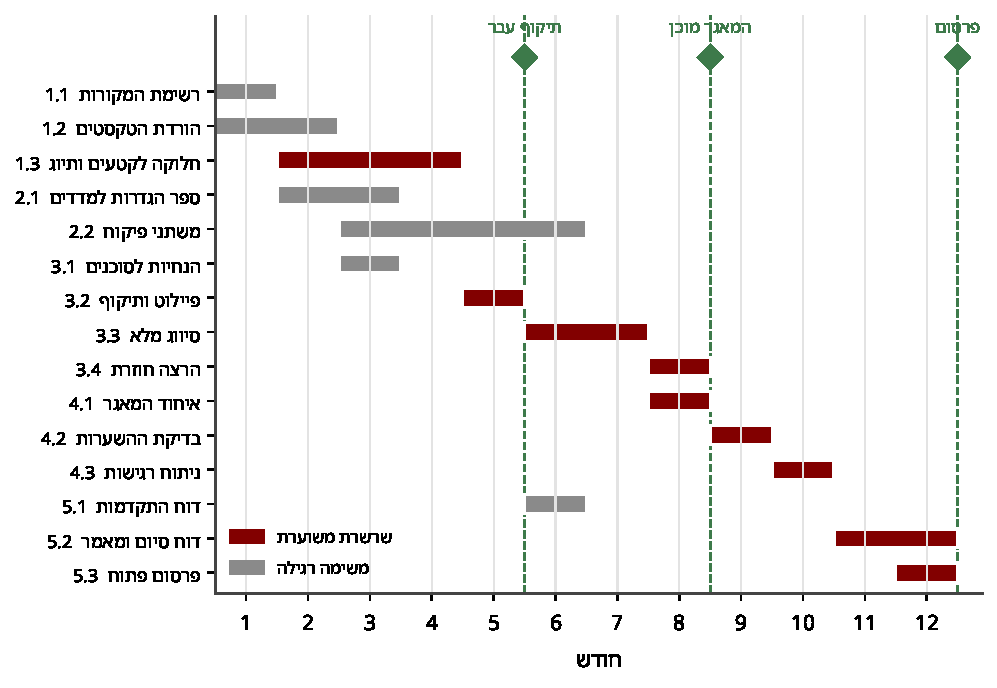
\includegraphics[width=0.92\textwidth]{figures/ch6-gantt.pdf}
  \caption{תרשים גאנט: 12 חודשים, שרשרת התלויות המשוערת באדום ושלוש אבני דרך בירוק}
  \label{fig:gantt}
\end{figure}

\paragraph{משמעות התלויות.} ציר החודשים הוא ברזולוציה גסה, וחלק מן המשימות נמסרות באצוות: רשימת ליבה מאושרת בחודש 1 מאפשרת התחלת הורדה, וטיוטת קידוד מאושרת מאפשרת הכנת הנחיות ואיסוף משתני פיקוח לפני סיום כל העדכונים. בחודש 8 בדיקת העקביות תסתיים לפני אישור המאגר; בחודש 12 הגרסה הסופית תינעל לפני הפרסום. אין להסיק מן החפיפה שכל תוצר סופי זמין בתחילת החודש. זו תוכנית תלויות מקדימה ולא חישוב \en{CPM} מלא; תאריכי המסירה, משכי העבודה ומרווחי הביטחון ייקבעו בתוכנית שבועית לפני ביצוע.

\paragraph{הנתיב הקריטי המשוער.} האדום מסמן שרשרת משוערת של אבני דרך תלויות: חלוקת הטקסטים לקטעים, הפיילוט והתיקוף, הסיווג המלא, בדיקת העקביות, איחוד המאגר, בדיקת ההשערות, ניתוח הרגישות, כתיבת דוח הסיום והפרסום. ההנחה היא שקיימת גמישות מסוימת במשימות כגון איסוף משתני הפיקוח ודוח ההתקדמות; היקפה טרם חושב, וכל שינוי ייבחן מול מועדי המסירה.

\paragraph{שלוש אבני הדרך.}
\begin{itemize}
  \item \textbf{סוף חודש 5: התיקוף עבר.} זו אבן הדרך החשובה ביותר: אם סיווגי המודל אינם עומדים ביעד של 85\%, אי אפשר להמשיך לסיווג המלא. לכן היא ממוקמת מוקדם, כשעוד יש זמן לתקן (פרק~\ref{ch:risks}).
  \item \textbf{סוף חודש 8: המאגר מוכן.} כל הנתונים – הסיווגים ומשתני הפיקוח – נמצאים במאגר אחד ועברו בדיקת שלמות (\en{REQ-DATA-01}).
  \item \textbf{סוף חודש 12: פרסום.} דוח הסיום, המאמר, והקוד והנתונים בגישה פתוחה.
\end{itemize}

\paragraph{מה קורה אם הפיילוט נכשל.} התיקוף נמצא על הנתיב הקריטי, ולכן כישלון שלו יעכב את כל המחקר. זו הסיבה שהוא ממוקם מוקדם ככל האפשר – בחודש החמישי, ולא לקראת הסוף. סבב תיקון ומבחן חדש צפויים לדרוש כחודש נוסף לפי הנחת התכנון. משום שהמשימה קריטית, אין בתוכנית מרווח שמבטיח ספיגה אוטומטית של העיכוב. במקרה כזה תוגש תוכנית מעודכנת: הקבלה של כתיבה וניתוח, צמצום היקף מאושר או הארכת לוח הזמנים. התוכנית לצמצום העיכוב הזה, ותוכנית המגירה אם גם הסבב השני ייכשל, מפורטות בפרק~\ref{ch:risks}.


\section{תקציב ומשאבים}
\label{sec:wp-budget}

טבלה~\ref{tab:budget} מציגה תקציב תכנון, לא הצעת מחיר מספק ולא הוצאה שכבר בוצעה. שני החוקרים מתוכננים להשקיע עשר שעות בשבוע כל אחד במשך 48 שבועות, בסך 960 שעות. לצורך השוואת חלופות בלבד הוערכה שעת חוקר ב־80 ש״ח ושעת מומחה ב־250 ש״ח. אלה הנחות תקציביות לאישור. הקצאת 70 שעות מומחה כוללת פיתוח קידוד, תיוג 450 קטעים, בדיקה כפולה של 60 קטעים והכרעת מחלוקות; היא תיבחן מחדש לאחר מיני־הפיילוט.

\begin{table}[htbp]
  \centering
  \caption{תקציב תכנון בש״ח לפי הנחות משאבים}
  \label{tab:budget}
  \small
  \begin{tabular}{p{48mm}p{51mm}r}
    \toprule
    \textbf{רכיב} & \textbf{בסיס החישוב} & \textbf{עלות} \\
    \midrule
    זמן שני החוקרים & \en{960 $\times$ 80} & \en{76,800} \\
    מומחה ותיוג נוסף & \en{70 $\times$ 250} & \en{17,500} \\
    שירותי מודלים & תקרת הקצאה לתכנון & \en{1,000} \\
    אחסון וגיבוי & תקרת הקצאה לתכנון & \en{1,000} \\
    \midrule
    סה״כ לפני עתודה & סכום ארבעת הרכיבים & \en{96,300} \\
    עתודה & \en{15\%} מהסכום & \en{14,445} \\
    \textbf{סה״כ כלכלי} & כולל זמן החוקרים & \en{110,745} \\
    \bottomrule
  \end{tabular}
\end{table}

אם זמן החוקרים ניתן כתרומה אקדמית ללא תשלום, התקציב הכספי המתוכנן הוא 19,500 ש״ח לפני עתודה ו־22,425 ש״ח אחריה. אין בכך התחייבות למימון. לפני שלב הביצוע יאושרו זמינות המומחה, התעריפים והתקרה. שינוי בשעות התיוג או שימוש בקידוד ידני יחייב עדכון משותף של התקציב ולוח הזמנים.

עלות המודל תיאמד מתוך 50 קטעי המיני־פיילוט: מספר טוקני קלט ופלט ממוצע לקטע, כפול מספר הקטעים, ההרצות וסוכני הבדיקה, במחירי המודל שנבחר ביום האישור. ב־80\% מניצול תקרת 1,000 הש״ח תופסק הרצה חדשה עד לבחינה מחדש. יעד של 2,000 קטעים מתויגים נשאר בתוקף גם אם חלק מהתיוג יועבר למסלול ידני; הקטנתו מחייבת אישור שינוי דרישה.
